\documentclass{article}

%in that file you will find the packages and other macro needed like \R for the real number set. 
\usepackage{vmargin}
\setmarginsrb{28mm}{25mm}{28mm}{25mm}{0pt}{0mm}{0pt}{0mm}
\setlength{\footskip}{20pt}
\usepackage{amssymb}
\usepackage{amsmath}
\usepackage{amsthm}
\usepackage{pgfplots} 
\usepackage{graphicx}
\usepackage[utf8x]{inputenc}
\usepackage{tikz}
\usepackage{bbm}
\usepackage{subcaption}
\usepackage[boxruled]{algorithm2e}
\usepackage{mathtools}
\usepackage{lipsum}
\usepackage[title,titletoc]{appendix}
\usepackage{booktabs}
\usepackage{here}
\usepackage[]{hyperref}
\usepackage{natbib,enumerate} 

%some weird packages
\usepackage{halloweenmath}
\usepackage{txfonts}
\usepackage{knitting}

\DeclarePairedDelimiter{\ceil}{\lceil}{\rceil}
\renewcommand{\phi}{\varphi}
\newcommand{\eqtext}[1]{\ensuremath{\stackrel{#1}{=}}}
\newcommand{\leqtext}[1]{\ensuremath{\stackrel{#1}{\leq}}}
\newtheorem{theorem}{Proposition}[section]
\newtheorem{lemma}{Lemma}[section]
\newtheorem{remark}{Remark}[section]
\newcommand{\N}{\mathbb{N}}
\newcommand{\R}{\mathbb{R}}
\newcommand{\E}{\mathbb{E}}
\newcommand{\epl}{\varepsilon}


\date{\today}

\begin{document}

%this creates the title page. You must complete the information there
\begin{titlepage}
    \newcommand{\HRule}{\rule{\linewidth}{0.5mm}} % Defines a new command for the horizontal lines, change thickness here
    
    \center % Center everything on the page
     
    %----------------------------------------------------------------------------------------
    %   HEADING SECTIONS
    %----------------------------------------------------------------------------------------
    
    \vspace{3cm}
    \textsc{\LARGE École polytechnique fédérale de Lausanne}\\[1.5cm] % Name of your university/college
    \textsc{\Large Semester project}\\[0.5cm] % Major heading such as course name
    \textsc{\large Master in Computational science and Engineering}\\[0.5cm] % Minor heading such as course title
    
    %----------------------------------------------------------------------------------------
    %   TITLE SECTION
    %----------------------------------------------------------------------------------------
    
    \HRule \\[0.4cm] % line above and under the title
    { \huge \bfseries Automatic vectorization of the  \\ renovated cadastre of Lausanne}\\[0.4cm] % Title of your document
    \HRule \\[1.5cm]
     
    %----------------------------------------------------------------------------------------
    %   AUTHOR SECTION
    %----------------------------------------------------------------------------------------
    
    \begin{minipage}{0.4\textwidth}
    \begin{flushleft} \large
    \emph{Author:}\\
    Danyang \textsc{Wang} % Your name
    \end{flushleft}
    \end{minipage}
    ~
    \begin{minipage}{0.4\textwidth}
    \begin{flushright} \large
    \emph{Supervisor:} \\
    Rémi \textsc{Guillaume Petitpierre}
    Frederic \textsc{Kaplan} % Supervisor's Name
    \end{flushright}
    \end{minipage}\\[10cm]
    
    %----------------------------------------------------------------------------------------
    %   LOGO SECTION
    %----------------------------------------------------------------------------------------
    
    
\includegraphics[width=0.4\linewidth]{Logo}\\[1cm] % Include a department/university logo - this will require the graphicx package
     
    %----------------------------------------------------------------------------------------
    
    \vfill % Fill the rest of the page with whitespace
    
    \end{titlepage}
    

\clearpage
\thispagestyle{empty}
\tableofcontents

\clearpage
\pagenumbering{arabic}
\setcounter{page}{1}

\section{Introduction}
In this project we analyse a model for describing the trajectory of particles of pollutants in groundwater. A successful model for describing underground flows is given by the uncertain Darcy problem. Given a domain $D$ such that its boundary $\partial D$ is divided in three subsets $\Gamma_{\rm in}, \Gamma_{\rm out}, \Gamma_N$ such that 
\begin{equation*}
	\Gamma_{\rm in} \cup \Gamma_{\rm out} \cup \Gamma_N = \partial D, \quad \Gamma_{\rm in} \cap \Gamma_{\rm out} \cap \Gamma_N = \emptyset,
\end{equation*} 
the pressure and velocity fields $p$ and $u$ are given by the solution of the following Partial Differential Equation (PDE)
\begin{equation}
	\label{eq:IntroDarcy}
	\left \{
	\begin{aligned}
		u &= -A \nabla p, && \text{in } D, \\
		\nabla\cdot u &= f, && \text{in } D, \\
		p &= p_0, && \text{on } \Gamma_{\rm in},\\
		p &= 0, && \text{on } \Gamma_{\rm out}, \\
		\nabla p \cdot n &= 0, && \text{on } \Gamma_N,
	\end{aligned} \right.
\end{equation}
where $\Gamma_{\rm in}$, $\Gamma_{\rm out}$ are the inlet and outlet portions of the boundary of $D$, and an impermeability condition is imposed on $\Gamma_N$.

\section{Title of section}
Let $D$ be a subset of $\R^d$ and $W(t)$ be a vector of $m$ independent Brownian motions and two functions $f\colon \mathbb{R}^d \rightarrow \R^d, g \colon \R^d \rightarrow \R^{d\times m}$. We consider the following stochastic differential equation (SDE)
\begin{equation}\label{eq:GeneralModel}
\left \{
\begin{aligned}
dX(t) &= f(X(t)) dt + g(X(t))dW(t), && 0 < t \leq T, \\
X(0)  &= X_0, && X_0 \in D.
\end{aligned} \right .
\end{equation}
The problem is equipped with two different types of boundary conditions, namely
\begin{itemize}
	\item[i.] some item
	\item[ii.] another one
\end{itemize}

\subsection{Title of subsection}

Look at the appendix. but also let us cite some famous mathematicians, such as  \citet{Eul1795}, \citet{Fisher:1950} and \citet{Mir06}.

\subsubsection{Title of subsubsection}

Some figures of the MA building at EPFL. 

\begin{figure}[h]
	\begin{subfigure}[b]{.5\textwidth}
		% include first image
		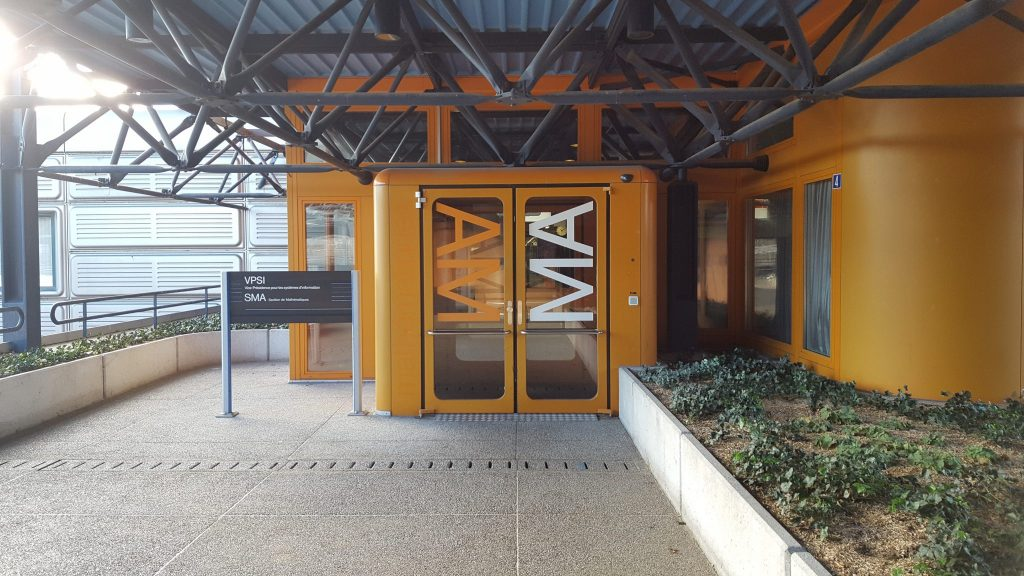
\includegraphics[width=.8\linewidth]{exterieur}  
		\caption{Put your sub-caption here}
		\label{fig:sub-first}
	\end{subfigure}
	\begin{subfigure}[b]{.5\textwidth}
		% include second image
		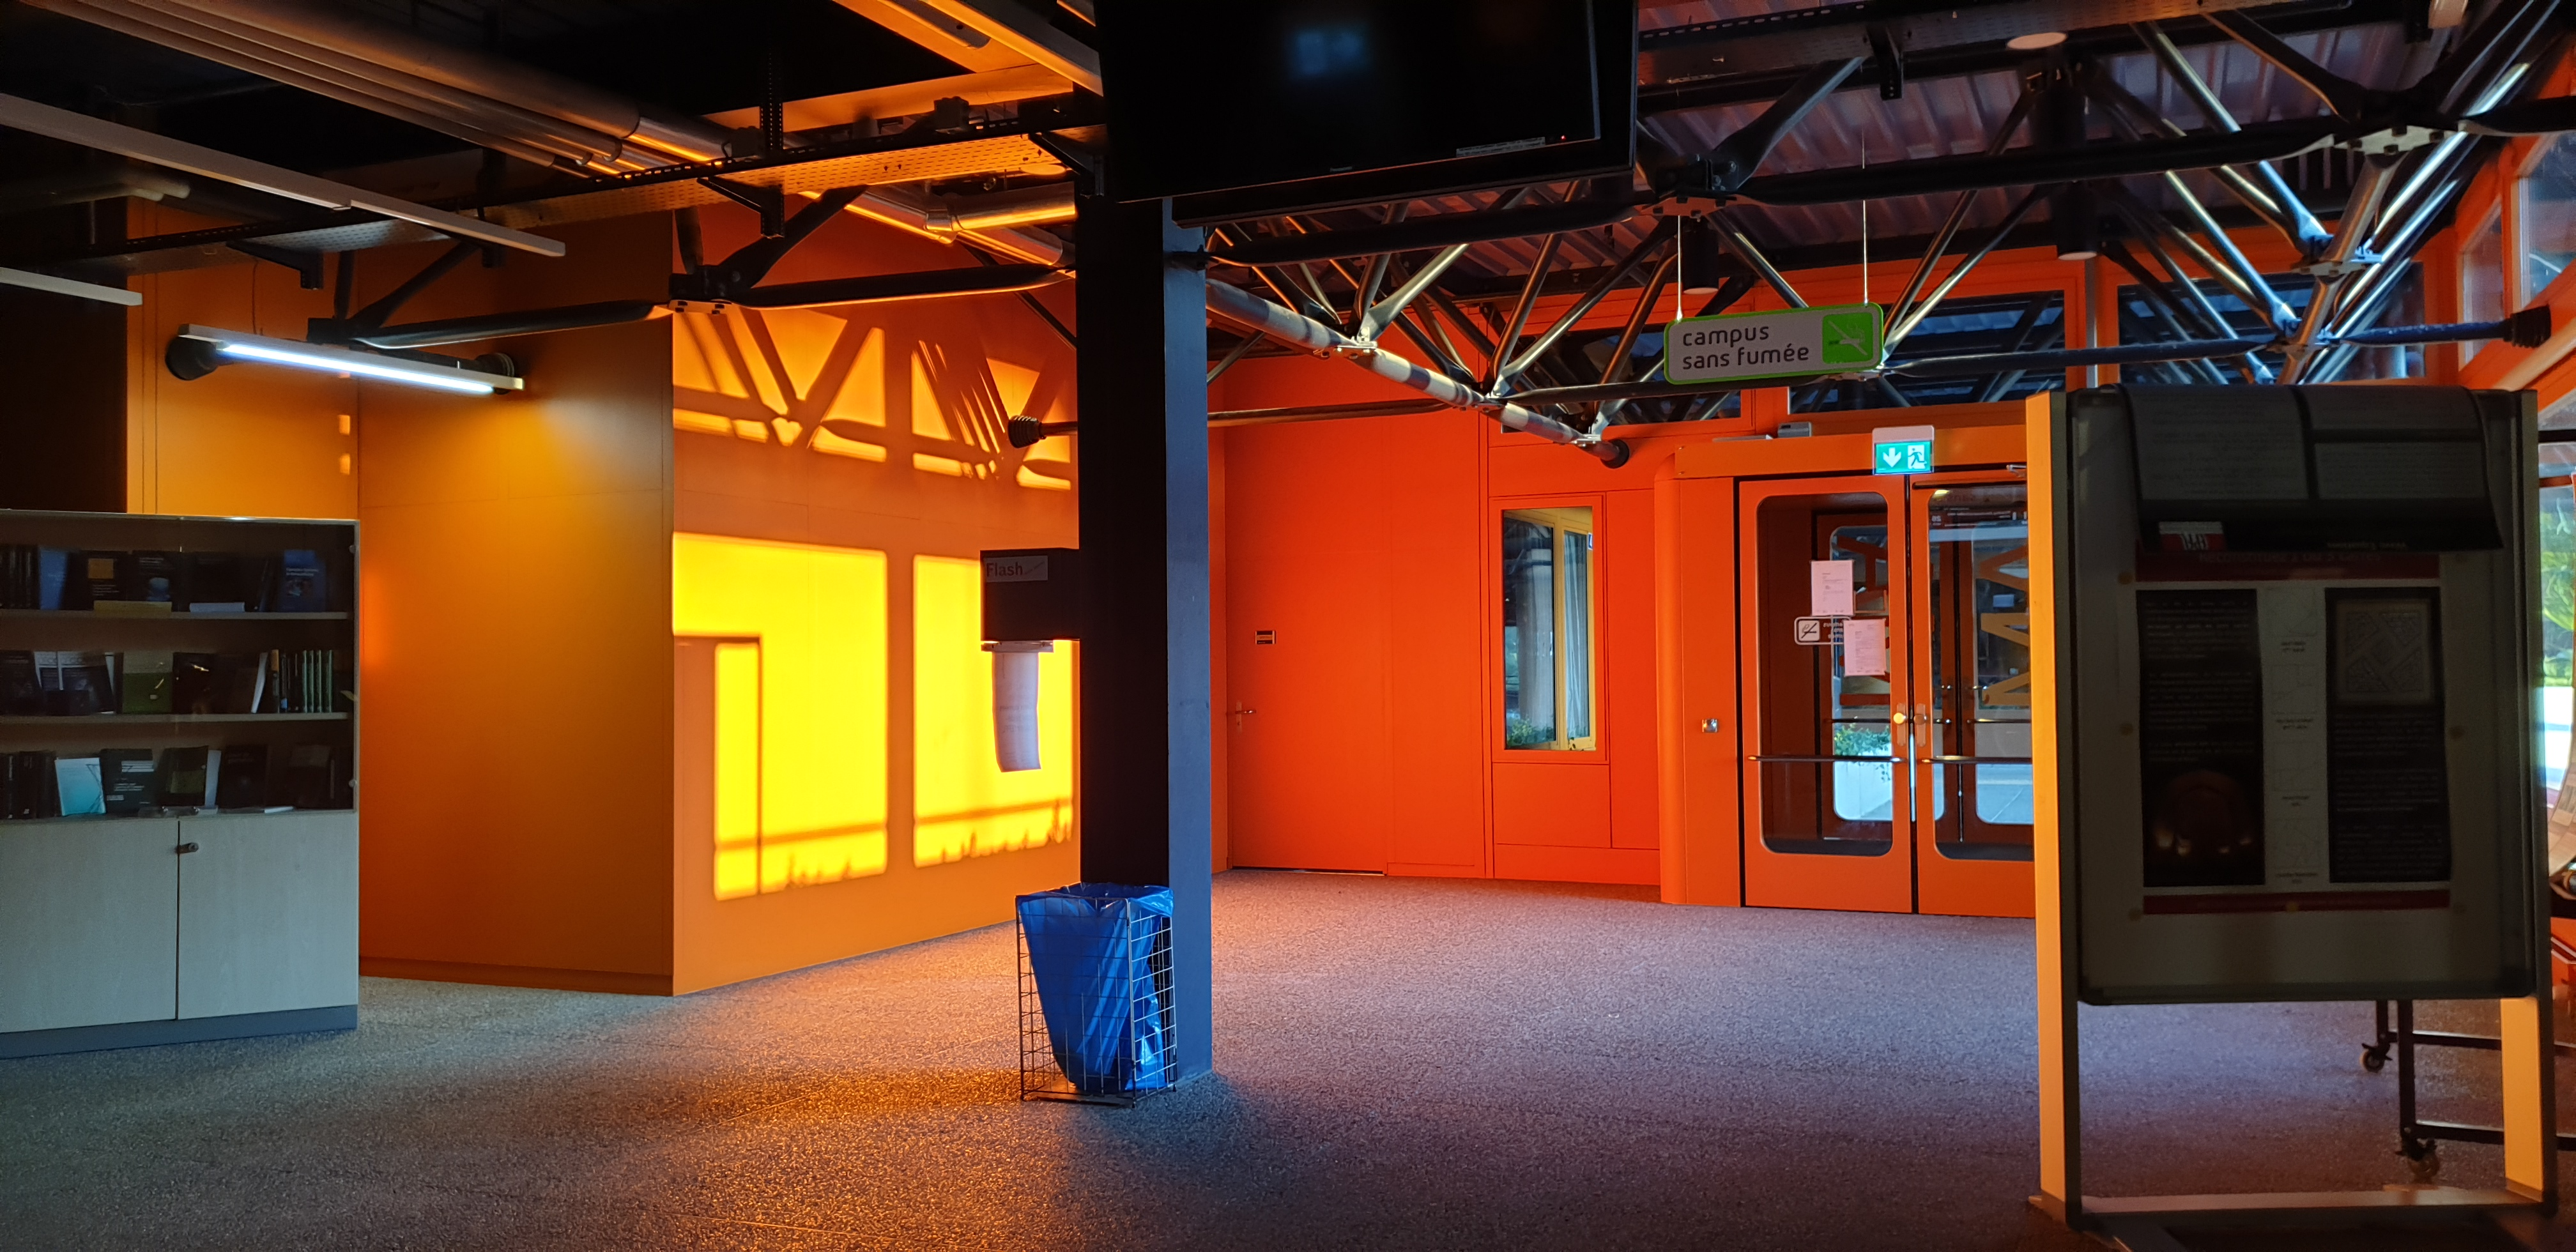
\includegraphics[width=.8\linewidth]{interieur}  
		\caption{Put your sub-caption here}
		\label{fig:sub-second}
	\end{subfigure}
	\caption{Put your caption here}
	\label{fig:fig}
\end{figure}
\section{Conclusion}

In this project we did a lot of things.

\clearpage
\begin{appendices}
\section{Symbols}
In the \href{http://tug.ctan.org/info/symbols/comprehensive/symbols-a4.pdf}{The Comprehensive \LaTeX \, Symbol List}, one can find a \textbf{lot} of symbols. Such as

$\therefore
\textknit{b} \ointclockwise$ $\leftrightsquigarrow$ $\looparrowleft$
or even some non-maths ones $\mathghost \mathwitch*$

\section{Using tikz for drawing}

Tikz can help you draw some nice things. but other tools exist as well. Take a look at  \href{http://math.et.info.free.fr/TikZ/bdd/TikZ-Impatient.pdf}{Tikz pour l'impatient}

Some examples:

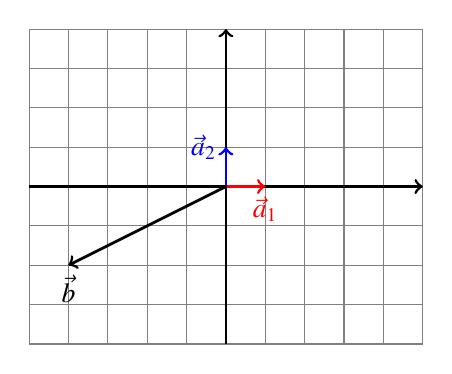
\begin{tikzpicture}
		\draw[gray] (-2.5,-2) grid[step=.5cm] (2.5,2);
		\draw[->, line width=1pt](-2.5,0)--(2.5,0);
		\draw[->, line width=1pt](0,-2)--(0,2);
		\draw[->, line width=1pt, red](0,0)--(1/2,0)coordinate (a);
		\draw[red] (a) node[below] {$\vec{a}_1$};
		\draw[->, line width=1pt, blue](0,0)--(0,1/2)coordinate (b);
		\draw[blue] (b) node[left] {$\vec{a}_2$};
		\draw[->, line width=1pt](0,0)--(-2,-1)coordinate (c);
		\draw[] (c) node[below] {$\vec{b}$};
\end{tikzpicture}

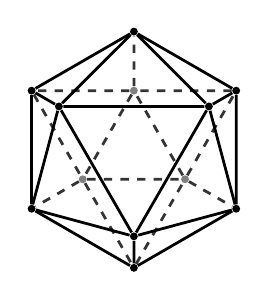
\begin{tikzpicture}
	\begin{scope}[scale=0.5, shift={(0,0)}, transparency group, color=black]
		\tikzstyle{every node}=[circle,fill=black,inner sep=0pt,minimum size=.1cm]
		\foreach \y[count=\a] in {10,9,4}
		{\pgfmathtruncatemacro{\kn}{120*\a-90}
			\node at (\kn:3) (b\a) {}
			;}
		\foreach \y[count=\a] in {8,7,2}
		{\pgfmathtruncatemacro{\kn}{120*\a-90}
			\node at (\kn:2.2) (d\a) {};}
		\foreach \y[count=\a] in {1,5,6}
		{\pgfmathtruncatemacro{\jn}{120*\a-30}
			\node[black!50] at (\jn:1.5) (a\a) {};}
		\foreach \y[count=\a] in {3,11,12}
		{\pgfmathtruncatemacro{\jn}{120*\a-30}
			\node at (\jn:3) (c\a) {};}
		\draw[dashed,line width=1pt,opacity=.8] (a1)--(a2)--(a3)--(a1);
		\draw[line width=1pt] (d1)--(d2)--(d3)--(d1);
		\foreach \a in {1,2,3}
		{\draw[dashed,line width=1pt,opacity=.8] (a\a)--(c\a);
			\draw[ line width=1pt] (d\a)--(b\a);}
		\draw[line width=1pt] (c1)--(b1)--(c3)--(b3)--(c2)--(b2)--(c1);
		\draw[line width=1pt] (c1)--(d1)--(c3)--(d3)--(c2)--(d2)--(c1);
		\draw[dashed,line width=1pt,opacity=.8] (b1)--(a1)--(b2)--(a2)--(b3)--(a3)--(b1);
\end{scope}	\end{tikzpicture}

\end{appendices}

\clearpage
\bibliography{biblio.bib}
\bibliographystyle{CUP}    % author-year citation style
% \bibliographystyle{siam}  % numbered citation style (deprecated by some)

\end{document}

